%!TEX program = lualatex
% Arquivo: Template_Estat_Texto.tex

\documentclass[a4paper,12pt]{article}

% =========================================================
% Idioma e tipografia (LuaLaTeX)
% =========================================================
\usepackage[portuguese]{babel}
\usepackage{fontspec}
\setmainfont{Latin Modern Roman}

% =========================================================
% Layout
% =========================================================
\usepackage[top=3cm,bottom=2.5cm,left=3cm,right=2.5cm]{geometry}
\usepackage{setspace}
\onehalfspacing
\usepackage{indentfirst}
\setlength{\parindent}{1.25cm}

% =========================================================
% Matemática (align*, etc.)
% =========================================================
\usepackage{amsmath}
\usepackage{amssymb}
\usepackage{siunitx}

% =========================================================
% Tabelas, listas, figuras
% =========================================================
\usepackage{booktabs}
\usepackage{array}
\usepackage{enumitem}
\setlist[itemize]{noitemsep,topsep=3pt}
\setlist[enumerate]{noitemsep,topsep=3pt}

\usepackage{graphicx}
\usepackage{float}
\usepackage{pdflscape}
\graphicspath{{./}{./imagens/}{./figuras/}}

% =========================================================
% Links
% =========================================================
\usepackage{hyperref}
\usepackage{xurl}
\hypersetup{
  colorlinks=true,
  linkcolor=black,
  urlcolor=blue,
  citecolor=black,
  pdfauthor={},
  pdftitle={}
}

% =========================================================
% Texto de preenchimento (lorem)
% =========================================================
\usepackage{lipsum}

% =========================================================
% Dados da capa
% =========================================================
\newcommand{\Instituicao}{Universidade / Instituição}
\newcommand{\Curso}{Oceanodrafia -- Estatística II}
\newcommand{\Professor}{Professor: Maria Elvira}
\newcommand{\Aluno}{Aluno: José Mauro Xavier Elsas}
\newcommand{\Cidade}{Rio de Janeiro}
\newcommand{\Ano}{2026}

\title{\textbf{Título do Documento}}
\author{\Aluno}
\date{\Cidade --- \Ano}

\begin{document}

% =========================================================
% Capa (página de rosto)
% =========================================================
\begin{titlepage}
\centering
{\large \Instituicao \par}
\vspace{0.5cm}
{\large \Curso \par}
\vspace{1.0cm}

{\LARGE \textbf{Análise exploratória de dados} \par}
\vspace{0.6cm}
{\Large Altura de Alunos de uma turma \par}

\begin{figure}[H]
  \centering
  
\includegraphics[width=.3\linewidth]{./uerj.jpg}
\end{figure}

\vfill



\begin{flushright}
\Aluno\\
\Professor
\end{flushright}

\vspace{1.0cm}
{\Cidade --- \Ano \par}
\end{titlepage}

% =========================================================
% Sumário
% =========================================================
\tableofcontents
\newpage

% =========================================================
% Corpo do texto (exemplos)
% =========================================================
\section{Exercício}

Uma turma de 40 estudantes teve as suas alturas anotadas. A tabela abaixo traz os valores de altura de cada um dos alunos.

\begin{table}[H]
    \centering
\begin{tabular}{cc|cc}
  \toprule
\textbf{i} & 
\textbf{X} & 
\textbf{i} & 
\textbf{X}\\
\midrule
1 & 162 & 21 & 169 \\
2 & 164 & 22 & 155 \\
3 & 170 & 23 & 157 \\
4 & 160 & 24 & 164 \\
5 & 166 & 25 & 172 \\
6 & 163 & 26 & 154 \\
7 & 165 & 27 & 163 \\
8 & 157 & 28 & 165 \\
9 & 158 & 29 & 178 \\
10 & 169 & 30 & 165 \\
11 & 148 & 31 & 170 \\
12 & 159 & 32 & 171 \\
13 & 176 & 33 & 158 \\
14 & 163 & 34 & 150 \\
15 & 152 & 35 & 162 \\
16 & 166 & 36 & 166 \\
17 & 175 & 37 & 172 \\
18 & 157 & 38 & 158 \\
19 & 164 & 39 & 168 \\
20 & 172 & 40 & 164 \\
\bottomrule
\end{tabular}
\caption{Alturas de 40 alunos.}
\label{tab:alturas}
\end{table}

\section{Amplitude da série}

Sendo o valor máximo da série \SI{178}{cm} e o valor mínimo \SI{148}{cm}, a amplitude da série é dada por:

\[
A = 178 - 148 = \SI{30}{cm}
\]

\subsection{Número de classes}

Para o número de classes, podem ser usadas as expressões:

\[
N = 40
\]

\[
\begin{cases}
\sqrt{40} = 6,32, \\
1 + 3,3\log 40 = 6,28
\end{cases}
\]

Entretanto, para obter classes de mesma amplitude inteira e facilitar a construção da distribuição de frequências, adotaram-se 5 classes. Assim, a amplitude de classe é:

\[
A_c = \frac{A}{5} = \frac{30}{5} = 6
\]

Então, fazendo a separação das alturas por classes, temos:

\begin{table}[H]
  \centering
    \begin{tabular}{lrrr}
      \toprule
      Altura & $f_a$ & $f_i$ (\%) & $f_{ac}$ (\%)\\
      \midrule
      148 $\vdash$ 154 & 3  & 7,5  & 7,5 \\
      154 $\vdash$ 160 & 9  & 22,5 & 30,0 \\
      160 $\vdash$ 166 & 13 & 32,5 & 62,5 \\
      166 $\vdash$ 172 & 9  & 22,5 & 85,0 \\
      172 $\vdash$ 178 & 6  & 15,0 & 100,0 \\
      \midrule
      $\sum f_a$ & 40 & 100,0 & \\
      \bottomrule
    \end{tabular}
\caption{Distribuição de frequências das alturas dos alunos.}
\label{tab:freq_alturas}
\end{table}

\subsection{Histograma}

\begin{figure}[H]
  \centering
    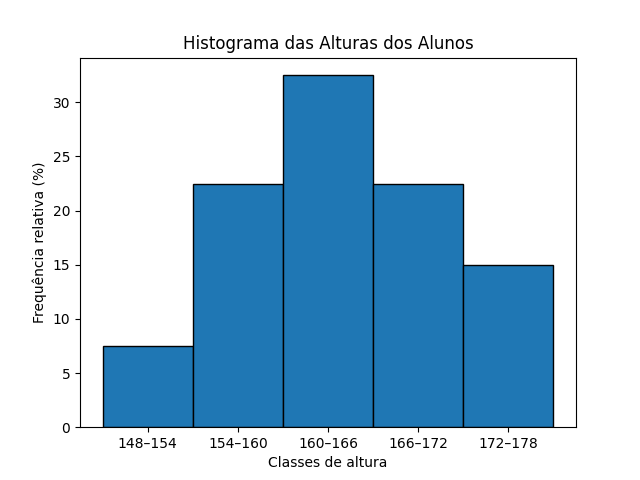
\includegraphics[width=0.9\linewidth]{./Figs/Histo_alturas.png}
  \caption{Histograma das alturas dos alunos.}
\end{figure}

\subsection{Frequências acumuladas}

\begin{figure}[H]
  \centering
    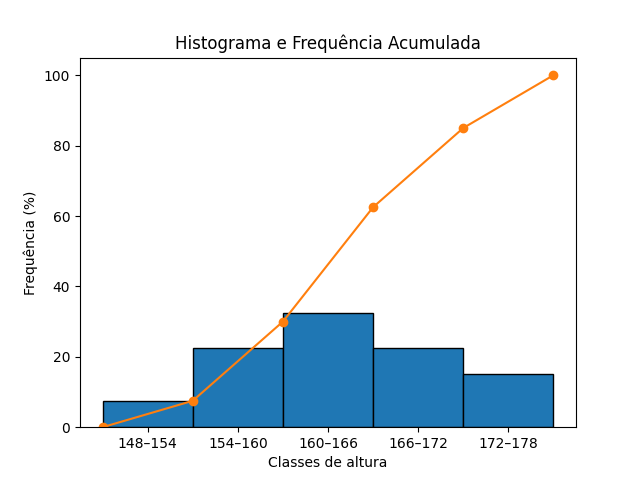
\includegraphics[width=0.9\linewidth]{./Figs/ogiva_e_acumulado.png}
  \caption{Ogiva das frequências acumuladas das alturas dos alunos.}
\end{figure}

\subsection{Estatíticas Descritivas}

\begin{tabular}{l}
Média =  163,68\\
Mediana =  164,00\\
Desvio padrão =  7,04\\
N = 40\\
Valor máximo = 178\\
Valor mínimo = 148\\
\end{tabular}


\end{document}